\section{Aufbau und Durchführung}
\label{sec:Durchführung}

Im folgenden werden die Messapparatur und die Vorgehen zur Bestimmung des magnetischen Moments beschrieben.

\subsection{Aufbau}

In der Mitte einer Billiardkugel befindet sich ein Permanentmagnet, dessen magnetisches Moment in Richtung des Stiels zeigt. 
Die Kugel bewegt sich wegen eines Luftkissens reibungsfrei auf einem Messingzylinder zwischen zwei Helmholtz-Spulen (Abbildung 3).  
Die zwei Helmholtz-Spulen ($N=195$) erzeugen ein Magnetfeld, und haben einen Abstand von $d=\SI{0.138}{\meter}$ und einen Radius von $R=\SI{0.109}{\meter}$.
Ein Stroboskop, welches sich an der oberen Spule befindet, bestimmt die Drehbewegung.
Mit einem Steuergerät können Strom, Magnetfeld, Stroboskop und Luftkissen eingestellt und bedient werden.

\begin{figure}[H]
  \centering
  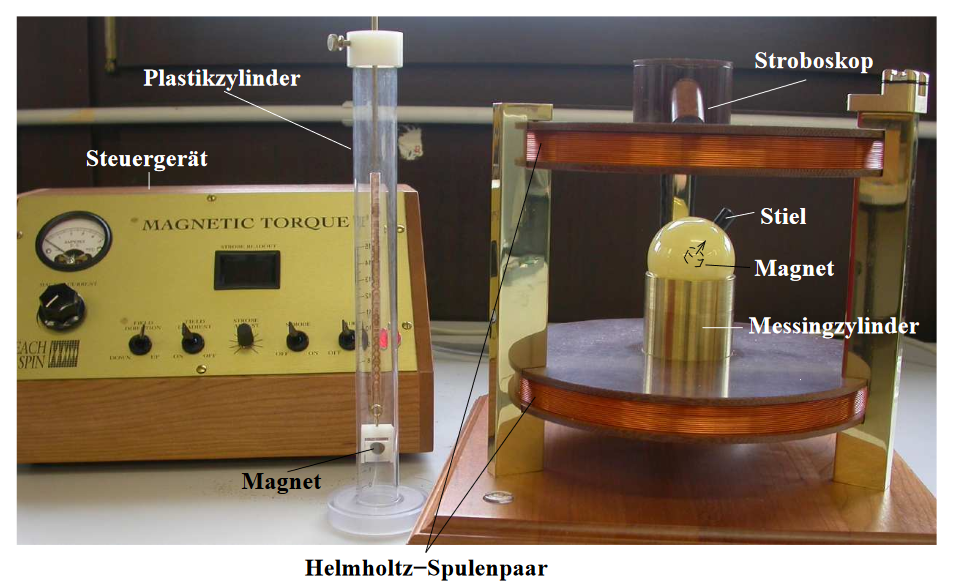
\includegraphics[height=8cm]{Screenshot (3).png}
  \caption{Versuchsaufbau mit Steuergerät, Helmholtz-Spulen und Billiardkugel. \cite[S. 2]{kent}}
  \label{fig:drill}
\end{figure}


\subsection{Durchführung}
Als erstes werden Radius und Masse der Billiardkugel gemessen und daraus das Trägheitsmoment bestimmt. Desweiteren wird die Länge des Stiels gemessen.

\subsubsection{Bestimmung des magnetischen Moments durch Gravitation}
In den Stiel der Kugel wird eine Aluminiumstange, auf welcher eine verschiebbare Masse ist, gesetzt, und die Kugel wird auf den Zylinder gesetzt.
Dann wird der Abstand $r$ von Anfang des Stiels bis zum Schwerpunkt der Masse bestimmt. 
Nun wird am Steuergerät das Gebläse für das Luftkissen eingeschaltet, die Feldrichtung auf ``up'' und der Feldgradient auf ``off'' gestellt.
Das Magnetfeld wird nun solange justiert, bis sich das System in einem Gleichgewicht befindet (Abbildung 4). 
Ist dies der Fall, werden sich Magnetfeld und Abstand notiert.
Diese Messung wird 10 mal wiederholt, wobei der Abstand beliebig verändert wird.

\begin{figure}[H]
  \centering
  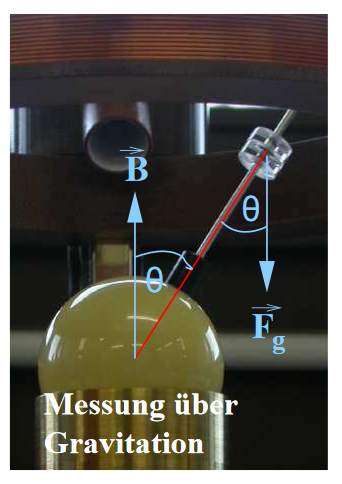
\includegraphics[height=5cm]{Screenshot (4)}
  \caption{Krafteinwirkungen auf Aluminiumstange und Masse. \cite[S. 3]{kent}}
  \label{fig:drill}
\end{figure}


\subsubsection{Bestimmung des magnetischen Moments durch Schwingungsdauer}

Wieder wird die Kugel auf den Zylinder gesetzt und das Magnetfeld eingeschaltet.
Die Kugel wird bei eingestelltem Magnetfeld nun in Schwingung versetzt, indem der Stiel um einen kleinen Winkel ausgelenkt wird.
Es werden 10 Perioden gemessen und die Ergebnisse gemittelt. Insgesamt wird dies für 10 Stromstärken wiederholt.


\subsubsection{Bestimmung des magnetischen Moments durch Präzession}

Es wird am Stroboskop eine Frequenz zwischen $\nu=\SI{4}{\hertz}$ und $\nu=\SI{6}{\hertz}$ eingestellt.
Die sich auf dem Zylinder befindende Kugel wird in Rotation versetzt und durch gezielte Berührungen ausgelenkt (Abbildung 5), 
bis diese die eingestellte Frequenz erreicht.
Das ist der Fall, wenn der weiße Punkt auf dem Stiel stationär erscheint.
Anschließend wird das Magnetfeld eingeschaltet und die Umlaufzeit $T$ gemessen.
Insgesamt wird die Messung für 10 Magnetfeldstärken wiederholt.


\begin{figure}[H]
  \centering
  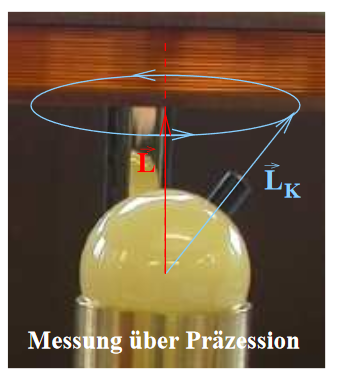
\includegraphics[height=5cm]{Screenshot (5).png}
  \caption{Achsenanordnung der Präzession. \cite[S. 5]{kent}}
  \label{fig:drill}
\end{figure}